\documentclass[12pt]{article}
\usepackage{amssymb}
\usepackage{amsmath}
\usepackage{amscd}
\usepackage{stmaryrd}
\usepackage{graphicx}
\setlength{\oddsidemargin}{.25in}
\setlength{\evensidemargin}{.25in}
\setlength{\textwidth}{6in}
\setlength{\textheight}{8.5in}
\hyphenpenalty = 10000
\pagenumbering{gobble}
\title{Cats and Dogs Recognition}
\author{Chongyuan Xiang, Min Zhang, and Weixin Chen}
\begin{document}
\maketitle
\begin{abstract}
In this paper, we focus on the problem of classifying images of cats and dogs, which is also known as one Asirra. We use three schemes to tackle the problem. First, we use information of the whole image; second, we use information of the animal body; third, we only use features from the head. The asymptotic behavior of the classification improves when we restrict the regions to the more distinguishable ones. We obtain 82.3$\%$, 84.4$\%$, and 85.6$\%$ under our best choice of features and voting scheme.  We anticipate that the accuracy of the second and third scheme will improve moderately if including more training samples.    
\end{abstract}


\section{Introduction}
The Asirra CAPTCHA $\cite{golle}$, proposed at ACM CCS 2007, relies on the problem of distinguishing images of cats and dogs (Asirra short for Animal Species Image Recognition for Restricting Access"). An Asirra challenge consists of 12 images, each of which is of either a cat or a dog. To solve the CAPTCHA, the user must select all the cat images, and none of the dog images. This is a task that humans are very good at. According to $\cite{golle}$, Asirra can be solved by humans 99.6$\%$ of the time in under 30 seconds. The usability of Asirra is a significant advantage compared to text recognition based CAPTCHAs. The preference towards Asirra is due to the presumed difficulty of classifying images of cats and dogs solely by machine. A classifier based on color features, described in $\cite{asirra}$, is only 56.9$\%$ accurate. $\cite{asirra}$ suggests classification accuracy of better than 60$\%$ will be difficult without a significant advance in the state of the art". However, with a 60$\%$ accurate classifier, the probability of solving a 12-image Asirra challenge is roughly 0.2$\%$. Later work on the field, for example $\cite{golle}$, has improved the specification of the feature vectors, which highly increases the probability of correctly classifying a single cat or dog image. In our work, we employ techniques, for example cascade procedure and image integral in $\cite{viola}$, from more general object detection settings, and combine them with promising feature vectors in the relevant research topics, in particular, HOG like features. We try different combination of color features and texture features to obtain a much better classifier under small training sample compared with those in $\cite{golle}$.

\section{Related Work}
$\cite{golle}$ proposes a classifier which is 82.7$\%$ accurate in telling part images of cats and dogs, which yields 10.3$\%$ odds in passing the 12-image Asirra task. Their choice of features are elegant yet straightforward, namely color and texture. The colors are interpreted in the hue-saturation-value (hsv) model, which is close to how people perceive colors. The other choice are red-green-blue (rgb), hue-saturation-light (hsl), and hue-saturation-intensity (hsi) models. We expect the choice of different models will generally affect the classifying results to some degree. Their color feature records the existence of a pixel with in some particular color region ($h,s,v$) in a cell. We adopt the same approach and try some variant models. Their texture feature, using the structural approach (will be explained in the texture feature section), mainly describe the variance of the colors of the image in the rob space. They achieve an accuracy of 82.7$\%$ by combining the SVM results of the two kinds of features with 8000 training examples on 2000 testing samples. However, we believe using other perspectives, in our case gradient features, of the image instead of rgb-cast colors will improve the classification. Our first texture features follow the statistical approach with similar underlying philosophy as $\cite{viola}$'s. We use the naive statistics, energy, contrast, correlation, and homogeneity (see section 3). The result is slightly worse than $\cite{goole}$. Considering the naivete and crudeness of the texture model, we anticipate a considerable ascendancy over []'s by refining our texture model. Improvement can be made by using more complicated features characterizing the texture, say the well known Histogram of Oriented Gradient (HOG), and BLP (binary local patterns). We do some test cases with training sample size ?? and testing sample size ??. The result is significantly better than [] with small sample sizes (xiangcy give example!!!!). There are three options. The first is to extract HOG, BLP of the whole image to run boosting, select a subset of most distinguishing features, and apply SVM. The second and third options ??? body and face??. The third option does a similar task as face detection. However, as commented in Zhang, Sun, and Tang [], applying the existing face detection approaches to detect the cat head is not feasible not only due to apparent greater appearance variations of cat faces compared to those of human faces, but also due to their more complicated textures. Same for dog faces. So it requires a different detection strategy. We tried the approaches in their paper. They used Haar of Histogram of Gradients as feature vector to train a detector for cat heads. The positive face examples are manually labeled out eyes and ears and normalized by aligning ears or eyes. However, normalizing the dog faces is much harder than cats because of larger variety of dog faces. Moreover, we are dealing with database with more diversity in face positions and directions. In particular, we took an approach mimicking the cascade ideas of Viola Jones $\cite{viola}$. Increasing layers has an considerable effect on reducing test errors -- in $\cite{viola}$, Viola and Jones trained a 37 layer decision tree to achieve over 85 percent performance, using thousands of positive examples and millions of negative examples. Due to limitation of time and machines, we use a decision tree of roughly 10 layers. Once we crop out heads from the original images, we use boost algorithm to train a classifier to classify cat heads and dog heads. This classifier will be much more accurate than classifiers directly trained from the whole image. In this part, we use HOOGs as our feature vectors. By training 200 cat heads and 200 dog heads, we get a classifier with performance higher than $90\%$.  

A trade off we made in our project is using Haar instead of HOG to train the cascaded decision tree. We tried on a small sample of images and found HOG is much more effective than Haar as feature vector. However, HOG is also much more intensive compared to Haar. Considering that there are tens of thousands of windows to be tested, the computation time of HOG will be unaffordable for this project, which makes us choose Haar as our feature vector. Computing the feature vectors require time??
The most interesting advantage of the Adaboost-based methods is its high accuracy
in dynamical environments, achieved with high processing speed.  Another interesting characteristic of the developed Adaboost-based methods is their relatively high training speed.


The usage of larger face sizes (48x48) slightly improves the performance of some methods (for example Adaboost-Rect features and Adaboost-Wav), however the training time increases exponentially (from hours to days).
Shape feature, which is used in $\cite{sun}$ to detect cat head, is also a first guess. It could have two usages: first, to crop out heads; second, to distinguish the dogs and cats. Although plausible at the first glance, the second usage was rejected once we realize there are cat-like dogs and dog-like cats, especially look alike in terms of shape. The first usage is not adopted in this project because it will take too long to train the classifier. As suggested by $\cite{sun}$,  cat ears

\section{Color Feature}
We first normalize all our pictures to be 250px$ \times $250px, then divide each picture into $n\times n$ square cells with equal size. Then we partition the color spaces. We use both RGB color space and HSV color space. In both of the color spaces, a color is represented by a triplet $(x,y,z)$. We normalize all these three values to be between 0 and 1. We then divide the $x,y,z$ coordinate into $N_x, N_y, N_z$ equal intervals, and the color space is divided into $N_x \times N_y \times N_z$ cubes. \\
We are now considering two features. The first feature $F_1(i, j)$ is an integer value. We go through all of the pixels inside the $i$-th cell of the picture, and then count the number of pixels whose colors are in the $j$-th cube of the color space. ($ 1 \leq i \leq n^2, 1 \leq j \leq N_x \times N_y \times N_z $), and the count is $F_1(i, j)$. The second feature $F_2(i, j)$ is a boolean value. We still go through all of the pixels inside the $i$-th cell of the picture. If among those pixels, there exists at least one pixel with color in the $j$-th cube of the color space, $F_2(i, j)$ is 1(true); otherwise, $F_2(i, j)$ is 0(false).\\
\begin{table}[h]
\caption{Color Feature Boosting Training Result}
\centering
\begin{tabular}{| l | l | l | l | l | l | l |}
\hline
Color Space Type & n & x & y & z & No. of weak learners & correction rate\\
\hline
RGB($x = r, y = g, z = b$) & 1 & 10 & 10 & 10 & 250 & $60.8 \%$\\
\hline
RGB($x = r, y = g, z = b$) & 3 & 10 & 10 & 10 & 250 & $71.9 \%$\\
\hline
HSV($x = h, y = s, z = v$) & 1 & 10 & 10 & 10 & 250 & $66.8 \%$\\
\hline
HSV($x = h, y = s, z = v$) & 1 & 10 & 10 & 10 & 500 & $66.7 \%$\\
\hline
HSV($x = h, y = s, z = v$) & 3 & 10 & 10 & 10 & 250 & $72.7 \%$\\
\hline
HSV($x = h, y = s, z = v$) & 5 & 10 & 10 & 10 & 250 & $72.7 \%$\\
\hline
HSV($x = h, y = s, z = v$) & 5 & 8 & 8 & 8 & 250 & $72.1 \%$\\
\hline
\end{tabular}
\end{table}
We choose to go with $F_2(i, j)$ because in the training pictures, the portion of the animal area varies. To classify a new picture, it makes more sense to check if the picture contains more typical dog colors or more cat colors instead of check the absolute number of pixels with typical dog colors or typical cat colors. \\
We use 10000 pictures to train our classifier, and then test 2000 pictures. We run boosting algorithm with a logistic loss.\\
From Table 1, we can see that the highest correction rate we achieve is 72.7 \%, with the feature HSV$(n =3 ,x = 10, y = 10, z = 10)$ or HSV$(n =5 ,x = 10, y = 10, z = 10)$. We can also notice that feature vector generated from HSV color space is better than feature vector from RGB color space.  A possible explanation is that HSV color space is more closer to human perception of color. 


\section{Texture Feature}
\subsection{GLCM}
We use Gray-Level Co-Occurence Matrix (GLCM) to analyse a picture's texture. In an $n \times n$ Gray-Level Occurence Matrix $G$, $G(i, j)$ represents how often a pixel with intensity $i$ occurs with an offset to a pixel with intensity $j$. \\
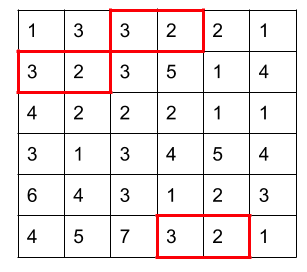
\includegraphics[width = 6cm]{glcm} \\
For example, the above shows the intensity level of each pixel in a 6-by-6 pixel images. If we set offset to be $(0,1)$, which means the second pixel is 0 pixel down and 1 pixel left comparing to the first pixel. We can see a pixel with intensity 3 occurs three times with this offset to a pixel with intensity 2. So $G(3,2) = 3$.\\
To get the GLCM, first, we transform the picture into a gray-level picture. Then each pixel should have its own intensity (gray-level). Then we use scaling to reduce the number of intensity values to be $n$, so we will get an $n \times n$ GLCM. and if we use $N_f$ offsets, we can get $N_f$ GLCMs. If the $o$-th GLCM matrix is $G_o$, our first texture feature $TF_1(o,i,j)$ represents $G_o(i, j)$. \\
Our second feature $TF_2$ will be the statistics of the GLCM instead of GLCM itself. $TF_2(o, i) (1 \leq i \leq 4)$ represent the $G_o$'s Contrast, Correlation, Energy and Homogeneity separately.
% Contrast is a measure of the intensity contrast between two neighbor pixels; Correlation is a measure of how correlated a pixel is to its neighbor; Energy is a measure of the whole image's intensity; Homogeneity is a measure of how close the elements in the GLCM are to the diagonal elements. 
Their definitions are given below: \\
$$ \mathrm{Contrast} = \sum_{i,j}|i-j|^2 G(i,j) ~~~~
 \mathrm{Correlation} = \sum_{i,j}\frac{(i - \mu_i)(j - \mu_j)G(i,j)}{\sigma_i \sigma_j} $$
$$ \mathrm{Energy} = \sum_{i,j}G(i,j)^2 ~~~~
\mathrm{Homogeneity} = \sum_{i,j} \frac{G(i,j)}{1 + |i-j|} $$
We also use the same 10000 pictures to train our classifier. Then we use our classfier to classify the same 2000 test pictures. For each picture, feature vector $TF_1$ has length $n^2 \times N_f$ and $TF_2$ has length $4 \times N_f$. And by $N_f =15$, the offsets are $(i,j) (0 \leq i, j \leq 3$ \& at least one of $i,j \neq 0)$. By $N_f = 24$, the offsets are $(i,j) (0 \leq i, j \leq 4$ \& at least one of $i,j \neq 0)$. Then we run boosting algorithm with a logistic loss and 250 weak learners.\\
From Table 2, we can see that all of the classifiers have similar correction rate. The highest correction rate we achieve is 67.1 \%, with the feature TF1$(n =8 ,N_f = 24)$ or TF1$(n =8 ,N_f = 15)$. We can also notice that TF1 feature (using GLCM matrix directly) is better than TF2 feature (using statistics of GLCM). One possible explanation is that only four statistics cannot show all the information of the picture. To improve this, we can add more statistics in the future, such as Dissimilarity and Entropy.

\begin{table}[h]
\caption{Texture Feature Boosting Training Result}
\centering
\begin{tabular}{| l | l | l | l | l | l | l |}
\hline
Feature Type & n & $N_f$ & correction rate\\
\hline
TF1 & 8 & 15 & $67.1 \%$\\
\hline
TF1 & 8 & 24 & $67.1 \%$\\
\hline
TF1 & 16 & 15 & $66.8 \%$\\
\hline
TF1 & 16 & 24 & $66.5 \%$\\
\hline
TF2 & 8 & 24 & $65.4 \%$\\
\hline
TF2 & 16 & 24 & $65.4 \%$\\
\hline
\end{tabular}
\end{table}

\subsection {HOOG}
HOOG is also a good feature to describe a picture's texture. A detailed discription of it is included in section 6.1.2. \\
 WEIXINC!!!



\section {Combination of Color and Texture Feature}
Assume that color feature vector has a length of $N_c$, the texture feature has a length of $N_t$. Our first approach is to concatenate the two feature vectors into a longer feature vector with a length of $N_c + N_t$. Then we will run boosting algorithm using the new feature vector. \\
The second approach is combining two classifiers instead of combing two feature vectors. Recall that for boosting classifier, each picture will have a voting. Assume that classfier 1 gives the picture a voting $v_1$, and classifier 2 gives the picture a voting $v_2$. Given parameter $\alpha$, we calculate a new voting $ v = \alpha \times v_1 + (1-\alpha) \times v_2$. We use different $\alpha$ to form different classifiers and use them to test on our training examples, and find one with the highest correction rate.
\begin{table}[h]
\caption{Combined Feature Training Result}
\centering
\begin{tabular}{| p{8cm}| l | l | l | l |}
\hline
Two feature vectors $F_1$ and $F_2$ & \multicolumn{4}{|c|}{Correction Rate} \\ \cline{2-5}
 & $F_1$ & $F_2$ & approach1 & approach2 \\
\hline
$F_1$ = RGB($n=1,x=10,y=10,z=10$), $F_2$ = TF1($n=16,N_f=24$) & 71.9\% & 66.5\% & 73.1\% & 73.8 \% \\
\hline
$F_1$ = HSV($n=3,x=10,y=10,z=10$), $F_2$ = TF1($n=8,N_f=24$) & 72.7\% & 67.1\% & 73.6\% & 74.5 \% \\
\hline
\end{tabular}
\end{table}\\
From Table 3, we can see that both of the approaches achieve a better correction rate, and approach 2 is better than approach 1. 


\section{Attack on Head Detection and Classification}
In this section, we will introduce some work we have done in cat and dog head detection and classification. Strictly speaking, we have not completely solve the problem due to time and computation limitations, but we did find this a possible approach for the original problem. Our goal is to build a head detector to find cat and dog head and then focus our attention on the head images to get a high performance classifier. The first step is to train a classifier to distinguish head and background images, using boost algorithms. We tried two kinds of feature vectors here: rectangular features and Haar of histogram oriented gradients and compared their performance. The second step is to build a `cascade' of classifiers to enhance the performance, especially reducing the false positive rate. Then, we simply search among all sub-windows in all scales, locations and directions in the image and using the cascade detector to test if the sub-window is a head. Notice that there would be thousands of sub-windows in a single image, thus rapid processing speed and extremely low false positive rate are two key points here. This is also the advantages of boost algorithms and the cascade technique -- boosting helps us select a small amount of `significant' features from a large amount of ones(usually over $10,000$) and cascade leads to low false positive rate. Finally, we train a classifier to classify cat heads and dog heads, using boost algorithms.


\subsection{Training Head Detector}
We have two sets of feature vectors to train our head detector- rectangular features, and HOG like features, for example HOG, EOH, and our choice is the combination of Haar and oriented gradients, known as HOOGs. $\cite{sun}$. While we generally believe the second sets of features yield higher accuracy in detecting the head, they are much more time consuming to compute feature vectors???? and running boosting. ??
  
\subsubsection{Rectangular Features}
The following figure comes from $\cite{viola}$, which demonstrates the canonical two-rectangle features, three-rectangle feature, and a four-rectangle feature, more or less capturing all rectangular features. We employ their technique of image representation, \textit{integral image}, to allows the features be computed very quickly. The same technique might be applied to the computation of HOOG features as well, but with limitation due to existence of multiple bins and renormalization procedure of HOOGs. So we do not use integral image to generate HOOGs.

XIANGCY add figure 1 in viola and jones.

\subsubsection{HOOG}
For image gradient $\vec{g}(x)$, given $K$ orientation bins, oriented gradients channel $g^k_0(x)$, $k = 1, \cdots, K$, is defined as $|\vec{g}(x)|$ if the orientation of $\vec{g}(x)$ agrees with $k$. Our two inspecting HOOG features are defined as followed. The in-channel feature and cross-channel feature are defined as 
\[HOOG^i(R_1,R_2, k) = \frac{S^k(R_1) - S^k(R_2)}{S^k(R_1) + S^k(R_2)}, ~~HOOG^c(R_1,R_2, k) = \frac{S^k(R_1) - S^{k+K/2}(R_2)}{S^k(R_1) + S^{k+K/2}(R_2)}.\]
\subsubsection{Boost Algorithms}
We manually cropped out 466 cat heads and 380 dog heads and generated 26000 background images. We tried both adaBoost and logitBoost. Result shows logitBoost is usually better than adaBoost, and such performance difference will be enlarged in the cascade process.

some result

Analysis of result. Not satisfying possibly because not aligned and normalized.
\subsection{Cascade of Classifier}
The idea is similar to a decision tree. At each layer of the cascade is a classifier and an example will be rejected immediately if it is rejected by one layer. When training the classifier, at each layer, we use boosting algorithms to select important features and find a reasonable threshold that almost all positive training examples will be left and a decent amount of negative training examples will be rejected. This way, negative examples will be rejected quickly while only a small number of positive examples will be misclassified. For the same reason, a large amount of negative examples are required. In $\cite{viola}$, Viola and Jones trained 9544 face images and 350 million background images to get a 37 layers of cascade classifier. In our project, we trained 400 cat heads, 400 dog heads, and 20 thousand background images with a 15 layers of cascade. We arrived at 4$\%$ false negative rate and $1\%$ false positive rate.   

some result compare adaboost and logtiboost compare different layers result

\subsection{Searching among Subwindows}

The universal technique is to test sub-windows with all possible location and sizes in the images and `merge' all positive sub-windows with close location and sizes. However, this requres a high performance classifier, usually with false positive rates in the magnitude of $10^{-4}$, because the large amount of negative sub-windows in the image. Since our classifier can only achieve 1\\
ADD SOME HEAD IMAGES HERE\\
Almost all results include part of head here. The problem is some are too big or too small. We expect that this can be improved by merging similar sub-windows which we did not have enough time to implement. Yet the current result is rather satisfying considering the small amount of training examples we used. We also found that the algorithm performs much better on image contains moderate size heads which often occupy 1/16-1/4 of the the original image size. This is reasonable as there are less sub-windows contains the head if head is too small or too large.
\subsection{Cat and Dog Classifcation}
Similar as training the head classifier, we use boosting algorithms with HOOG or rectangular features as our feature vector to classify cat heads and dog heads. We trained our classifier on 250 cat head images and 250 dog images and tested its performance on manually cropped heads and on machine cropped heads.

\section{Results}

\section{Conclusion}

\begin{thebibliography}{99}
\bibitem{viola} 
\bibitem{sun}
\bibitem{golle} 
\bibitem{asirra} J. Elson, J. Douceur, J. Howell and J. Saul. \textit{Asirra: a CAPTCHA that exploits interest-aligned manual image categorization.} In Proc. of ACM CCS 2007, pp. 366-374.
\end{thebibliography}
\end{document}
